\section{Zielsetzung}
In diesem Versuch wird das magnetische Moment durch drei verschiedene Methoden gemessen und bestimmt.

\section{Theorie}
Im Unterschied zum elektrischen Feld, besitzt das magnetische Feld keine Quellen. Es gibt nur magnetische Dipole, keine Monopole.
Dipole erzeugen geschlossene Feldlinien. Dipole können makroskopisch durch einen Permanentmagneten oder durch eine
stromdurchflossene Leiterschleife erzeugt werden. Die Leiterschleife besitzt dabei das magnetische Moment $\mu$,
was mit folgender Formel berechnet werden kann:

\begin{equation*}
\mu = I \cdot \vec{A}
\end{equation*}
Hierbei ist $I$ der Strom, der durch die Leiterschleife fließt und $A$ die Querschnittsfläche der Leiterschleife.
Im folgenden wird das magnetische Moment \mu eines Permanentmagneten, der sich im Innern einer Billardkugel befindet,
experimentell mittels dreier verschiedener Methoden ermittelt.
Zur Erzeugung eines homogenen Magnetfeldes wird im Experiment ein $Helmholtz-Spulenpaar$ verwendet. Hierbei sind
zwei gleich große, gleich geformte, gleichsinnig vom Strom $I$ durchflossene Spulen so angeordnet, dass der Abstand
zwischen den beiden Spulen annähernd ihrem Radius entspricht. Das somit vom Spulenpaar erzeugte Magnetfeld ist auf der
Symmetrieachse der beiden Spulen homogen und kann mittels des $Biot-Savart-Gesetzes$ berechnet werden:

\begin{equation}
\label{biotsavartgesetz}
\vec{B}(x) = \frac{\mu_0 I}{4\pi} \frac{\symup{d}\vec{s}\times{\vec{r}}}{r^3}
\end{equation}

Ist der Abstand zwischen den beiden Spulen nicht identisch mit dem Radius der beiden Spulen, so gibt es zur Berechnung
des Magnetfeldes folgende Formel, die für weitere Berechnungen verwendet wurde, da sich im Experiment der Radius der
Spulen geringfügig von deren Abstand unterschied:

\begin{equation*}
\vec{B}(x) = \frac{\mu_0 I}{2} \frac{R^2}{(R^2 + x^2)^\frac{3}{2}}
\end{equation*}

Hierbei beschreibt $R$ den Spulenradius und der Abstand der beiden Spulen voneinander beträgt $2x$.
Das gesamte Feld im Zentrum des Spulenpaares erfolgt durch Superposition der Einzelfelder.

\begin{equation*}
B(0) = B_1(x) + B_1(-x) = \frac{\mu_0 I R^2}{(R^2 + x^2)^\frac{3}{2}}
\end{equation*}

Hier wurde der Einfachheit halber das Zentrum des Spulenpaares in den Ursprung des Koordinatensystems gelegt.


\section{Durchführung}
Es gilt nun das magnetische Moment $\mu_\text{Dipol}$ einer Billardkugel, in der sich ein kleiner Permanentmagnet befindet auf drei verschiedene Arten
zu ermitteln:
\begin{enumerate}
\item Unter Ausnutzung der Gravitation \\
\item Unter Ausnutzung der Schwingungsdauer $T$ \\
\item Unter Ausnutzung der Präzessionsbewegung \\
\end{enumerate}
Zur Durchführung des Versuchs wird ein Helmholtz-Spulenpaar mit oben angegeben Werten für $R_\text{Spule}$, $N$ und $d$ verwendet. Im Zentrum des Spulenpaares
(beide kreisförmigen Spulen sind so angeordnet, dass sich das B-Feld senkrecht im Raum befindet) ist ein kleiner Messingzylinder befestigt, welcher
eine kugelförmige Aussparung besitzt, sodass er die Billardkugel ideal aufnehmen kann. Mittels eines Luftkissens kann sich die Billardkugel
reibungsfrei auf dem Zylinder bewegen. Das magnetische Moment der Billardkugel ist in Richtung eines kleinen Stiels gerichtet, welcher sich an der Kugel befindet.
An der Oberseite des Spulenpaares befindet sich ein Stroboskop, welches im Verlauf des Versuchs zur Bestimmung der Frequenz der Drehbewegung genutzt werden wird.
Der Strom und folglich auch das durch die Spulen erzeugte Magnetfeld, das Stroboskop und das Luftkissen können extern eingeschaltet werden.
Veränderbar ist hier die Stromstärke, die Frequenz, mit der das Stroboskop aufblitzt und die Feldlinienrichtung, wobei diese im Experiment nicht
verändert wird. Sie ist kontinuierlich auf "up" eingestellt, was besagt, dass die Feldlinien von unten nach oben ausgerichtet sind.\\
Für alle weiteren Berechnungen sind die Werte, als auch die Abmessungen für die Spulen und deren Abstand zueinander, die in der Versuchsvorbereitung
gegeben sind, weiterverwendet. Zu Beginn des versuches, sind diese noch auf Richtigkeit zu überprüfen.

\newpage

\subsection{Bestimmung des magnetischen Moments der Billardkugel unter Ausnutzung der Schwerkraft}

Bei dieser statischen Methode wird die Tatsache verwendet, dass eine Masse $m$, die der Schwerkraft $\vec{F} = m \cdot \vec{g}$
unterliegt, ein Drehmoment

\begin{equation}
  \label{DrehmomentGravitation}
\vec{D_g} = m \cdot (\vec{r} \times \vec{g})
\end{equation}

auf die Kugel ausübt. Das Gewicht, welches dieses Drehmoment ausüben soll,
ist im Versuch verschiebbar auf einem Aluminiumstab, der als masselos anzusehen ist, befestigt. Dieser Stab wiederum steckt im Stiel der Billardkugel.
Dem durch die Schwerkraft verursachten Drehmoment, wirkt das durch das B-Feld verursachte Drehmoment

\begin{equation}
  \label{DrehmomentMagnetfeld}
\vec{D_B} = \mu_\text{Dipol} \times \vec{B}
\end{equation}

entgegen.
Bei genau einer Magnetfeldstärke sind $\vec{D_g}$ und $\vec{D_B}$ gleich und die Kugel führt keine Pendelbewegung mehr aus. Ist dies der Fall, so wird
die eingestellte Stromstärke $I$ zur Berechnung des entstandenen B-Feldes, sowie der Abstand $r$, vom Mittelpunkt des Gewichts bis zur Billardkugel,
notiert. Dieser Vorgang wird neun mal wiederholt, um statistische Fehler klein zu halten. \\

\subsection{Bestimmung des magnetischen Momentes mit Hilfe der Schwingungsdauer T des Magneten}

Wird die Kugel im eingeschalteten B-Feld in Schwingung versetzt, so verhält sie sich wie ein harmonische Oszillator, dessen Bewegung wie folgt
beschrieben werden kann:
\begin{equation*}
  -\vert{\vec{\mu}_\text{Dipol} \times \vec{\symup{B}}}\vert = J_\text{K} \cdot \frac{\symup{d^2}\theta}{\symup{d}t^2}
\end{equation*}
Die Lösung der Differentialgleichung ergibt eine Gleichung für die Schwingungsdauer T:
\begin{equation*}
  \symup{T^2} = \frac{4\symup{\pi}^2 \symup{J}_\text{K}}{\mu_\text{Dipol}} \frac{1}{\symup{B}}
\end{equation*}
Mithilfe der vorher berechneten Größen für das Trägheitsmoment der Kugel $J_k$ und das B-Feld lässt sich nun das magnetische Moment
der Kugel berechnen.
Im Experiment werden pro eingestellter Stromstärke zehn Periodendauern gemessen. Dies wird für neun verschiedene Stromstärken durchgeführt.

\subsection{Bestimmung des magnetischen Moments über die Präzessionsbewegung der sich drehenden Billardkugel}

Wird die Billardkugel mit ihrem Stiel senkrecht nach oben zeigend in eine Rotationsbewegung versetzt und stößt sie danach mit einem kleinen Stoß gegen den Stiel
an, sodass sie aus der senkrechten Position ausgelenkt wird, so führt die Achse der Kugel, durch den Stiel gehend, im eingeschalteten B-Feld eine Präzessionsbewegung aus.
Dabei beschreibt die Achse der Kugel einen Kegelmantel um die Drehimpulsachse,senkrecht im Raum stehend. Durch die Rotation der Kugel bleibt deren Auslenkung stabil.
Die Differentialgleichung für die Präzessionsbewegung sieht wie folgt aus:
\begin{equation*}
  \mu_\text{Dipol} \times \vec{\symup{B}} = \frac{\symup{d}\vec{L_\text{K}}}{\symup{d}t}
\end{equation*}
Die Formel für die Präzessionsfrequenz $\symup{\Omega}_\text{p}$ ist eine Lösung der Differentialgleichung und lautet:
\begin{equation*}
  \Omega_\text{p} = \frac{\mu_\text{Dipol}\symup{B}}{\vert{\symup{L}_\text{K}\vert}}
\end{equation*}
$\symup{L}_\text{K}$ beschreibt den Drehimpuls der ausgelenkten Kugel und kann mit Hilfe des Trägheitsmomentes der Kugel und deren Kreisfrequenz
berechnet werden: $\symup{L}_\text{K} = \symup{J}_\text{K} \omega$ . \omega = 2 \pi \nu.
Somit kann $\mu_\text{Dipol}$ über die Formel
\begin{equation*}
  \frac{1}{\symup{T}_\text{p}} = \frac{\mu_\text{Dipol}}{2\symup{\pi}\symup{L}_\text{K}} \symup{B}
\end{equation*}
bestimmt werden. \\
Um eine konstante Rotationsfrequenz $\nu$ zu erreichen, wird das Stroboskop eingeschaltet. Nachdem die Kugel bei senkrecht stehendem Stiel in eine
Rotationsbewegung versetzt wird, betrachte man den auf dem Stiel eingezeichneten kleinen Punkt.
Erscheint der Punkt stationär, so hat die Billardkugel eine konstante Rotationsfrequenz und kann durch einen kleinen Stoß aus der senkrechten Achse
ausgelenkt werden. Ist dies geschehen, so wird schnellstmöglich das B-Feld eingeschaltet und die Zeit $\symup{T}_\text{p}$ für einen Umlauf des Stiels
gemessen werden. Um statistische Fehler zu minimieren, wird die Messung drei Mal pro Magnetfeldstärke und für insgesamt neun unterschiedliche
Magnetfelder durchgeführt.
\\


\newpage

\section{Auswertung}

\subsection{Messung des magnetischen Momentes durch die Gravitation}
Die gemessenen Stromstärke und der Radius sind in Tabelle \ref{tab:1} aufgelistet.

\begin{table}
  \centering
  \caption{Messwerte der Gravitationsmethode.}
  \label{tab:1}
  \begin{tabular}{c c}
  \toprule
  $I$ / \si{\ampere} & $r$ / \si{\centi\meter} \\
  \midrule
  1.7 & 5.100 \\
  2.0 & 6.080 \\
  2.3 & 6.585 \\
  2.5 & 8.055 \\
  2.6 & 7.720 \\
  2.9 & 8.875 \\
  3.2 & 9.650 \\
  3.5 & 10.360 \\
  3.8 & 11.480 \\
  \bottomrule
  \end{tabular}
  \end{table}

  \begin{figure}[h]
    \centering
    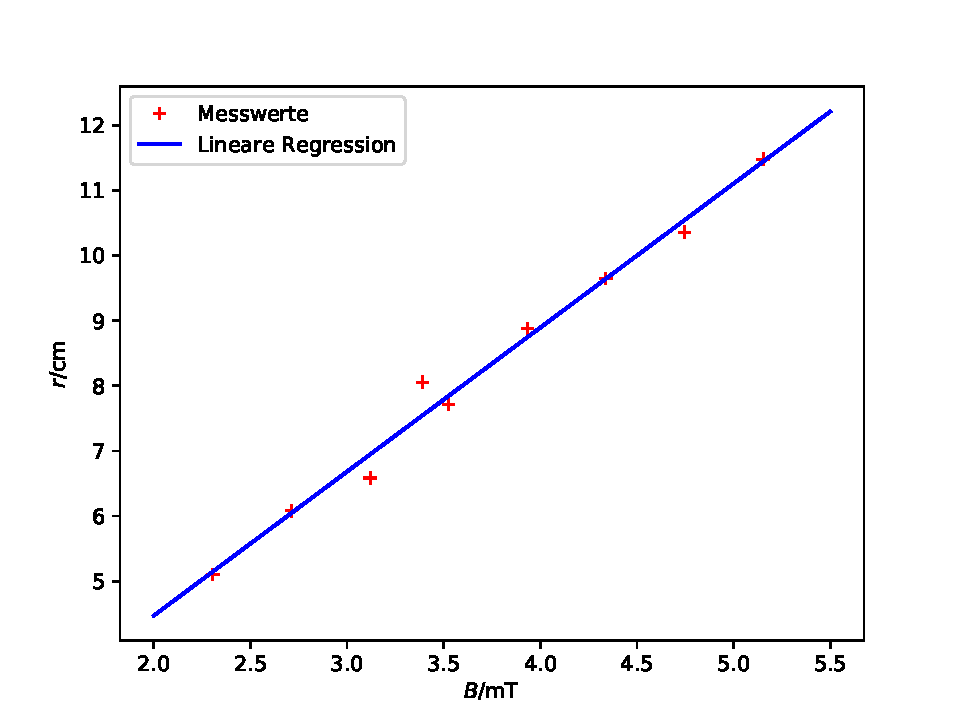
\includegraphics[scale=0.7]{Gravmet.pdf}
    \caption{Messwerte und lineare Regression der Gravitationsmethode.}
    \label{Abb:1}
  \end{figure}

Durch das Biot-Savart-Gesetz \eqref{biotsavartgesetz} und die gemessenen Stromstärken, lässt sich das Magnetfeld
im Mittelpunkt der Helmholzspule berechnen. In Abbildung \ref{Abb:1} wird das Magnetische Feld $B$ gegen den Radius
$r$ aufgetragen und eine lineare Regression durchgeführt.

Die lineare Regression setzt sich aus Folgenden Werten für die Steigung $m_1$ und für den y-Achsenabschnitt $n_1$ zusammen:

\begin{align*}
   m_1 &= \SI{2.21(10)}{\centi\meter\per\milli\tesla} \\
   n_1 &= \SI{0.0(4)}{\centi\meter}
\end{align*}

Durch Gleichsetzen der Drehmomente durch die Gravitation \eqref{DrehmomentGravitation} und durch das Magnetfeld \eqref{DrehmomentMagnetfeld},
ergibt sich die Steigung $m_1$ der linearen Regression, aus welcher sich das magnetische Moment berechnen lässt.

\begin{equation*}
  m_1 = \frac{\mu_\symup{Dipol 1}}{m_\symup{Dipol} \cdot g}
\end{equation*}

wobei

\begin{align*}
  m_\symup{Dipol} &= \SI{1.4}{\gram} \\
  g &= \SI{9.81}{\meter\per\second\squared}
\end{align*}

 iat. Nach Umformen der Gleichung ergibt sich das magnetische Moment des Dipols

 \begin{equation*}
   \mu_\symup{Dipol 1} = m_1 \cdot m_\symup{Dipol} \cdot g
 \end{equation*}

Durch Einsetzen der Werte folgt

\begin{equation*}
  \mu_\symup{Dipol 1} = \SI{30.35(137)e-2}{\ampere\meter\second}
\end{equation*}

Der Fehler wird mit der Gaußschen Fehlerfortpflanzung berechnet.

\begin{equation*}
  \Delta\mu_\symup{Dipol1} = m \cdot g \cdot \Delta m_1
\end{equation*}
\newpage

\subsection{Messung des magnetischen Momentes über die Schwingungsdauer eines Magnetes}

Die gemessenen Werte der Methode sind in Tabelle \ref{tab:2} aufgelistet.

\begin{table}
  \centering
  \caption{Messwerte der Methode durch die Schwingungsdauer}
  \label{tab:2}
  \begin{tabular}{c c c}
  \toprule
  $I$ / \si{\ampere} & 10$T$ / \si{\per\second} & $T$ / \si{\per\second} \\
  \midrule
  0.6 & 25.34 & 2.534 \\
  0.8 & 21.87 & 2.187 \\
  1.0 & 17.90 & 1.790 \\
  1.6 & 14.47 & 1.447 \\
  1.9 & 13.25 & 1.325 \\
  2.2 & 12.23 & 1.223 \\
  2.4 & 11.94 & 1.194 \\
  2.6 & 11.34 & 1.134 \\
  2.9 & 10.69 & 1.069 \\
  3.5 & 9.53 & 0.953  \\
  \bottomrule
  \end{tabular}
  \end{table}

  \begin{figure}[h!]
    \centering
    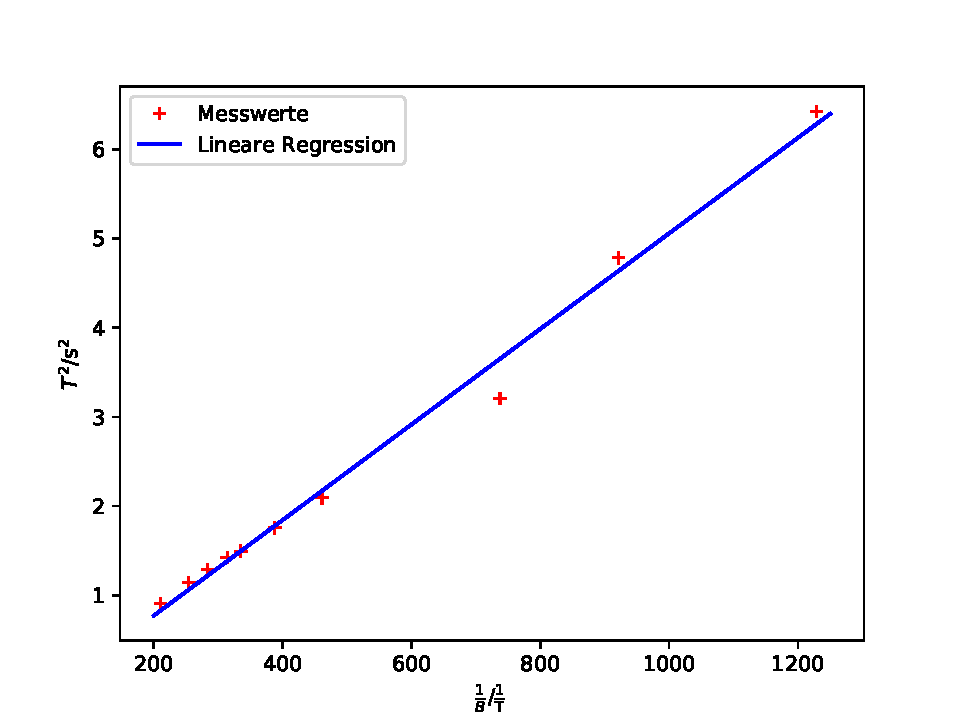
\includegraphics[scale=0.7]{Oszi.pdf}
    \caption{Messwerte und lineare Regression: Methode über die Schwingungsdauer.}
    \label{Abb:2}
  \end{figure}

In Abbildung \ref{Abb:2} wurde $T^2$ gegen $1/B$ aufgetragen. Durch eine lineare Regression kann dessen Steigung $m_2$
und dessen y-Achsenabschnitt $n_2$ ermittelt werden.

\begin{align*}
  m_2 &= \SI{5.35(18)e-3}{\second\squared\per\tesla} \\
  n_2 &= \SI{-0.30(11)e3}{\second\squared}
\end{align*}

Analog zur vorherigen Methode kann das Dipolmoment über die Steigung der linearen Regression bestimmt werden.

\begin{equation*}
  m_2 = \frac{4 \pi^2 J_k}{\mu_\symup{Dipol2}}
\end{equation*}

Wobei $J_k$ das Trägheitsmoment der Kugel ist, welches folgenden Wert besitzt:

\begin{equation*}
  J_k = \SI{3.75e-5}{\kilo\gram\meter\squared} .
\end{equation*}

Durch Umformungen und Einsetzen ergibt sich

\begin{equation*}
  \mu_\symup{Dipol2} = \frac{4 \pi^2 J_k}{m_2}
\end{equation*}

\begin{equation*}
  \mu_\symup{Dipol2} = \SI{27.67(93)e-2}{\ampere\meter\squared}
\end{equation*}

\newpage

\subsection{Bestimmung des magnetischen Momentes über die Präzession eines Magneten}

\begin{table}
  \centering
  \caption{Messwerte der Methode über die Präzession}
  \label{tab:3}
  \begin{tabular}{c c}
  \toprule
  $I$ / \si{\ampere} & $\overline{T}$ / \si{\second} \\
  \midrule
  0.5 & \num{28.50(331)} \\
  1.0 & \num{16.31(184)} \\
  1.5 & \num{10.90(30)} \\
  1.8 & \num{10.57(34)} \\
  2.0 & \num{10.24(41)} \\
  2.5 & \num{6.48(119)} \\
  3.0 & \num{5.56(28)} \\
  3.5 & \num{5.63(15)} \\
  3.9 & \num{5.26(47)} \\
  \bottomrule
  \end{tabular}
\end{table}

\begin{figure}[h]
  \centering
  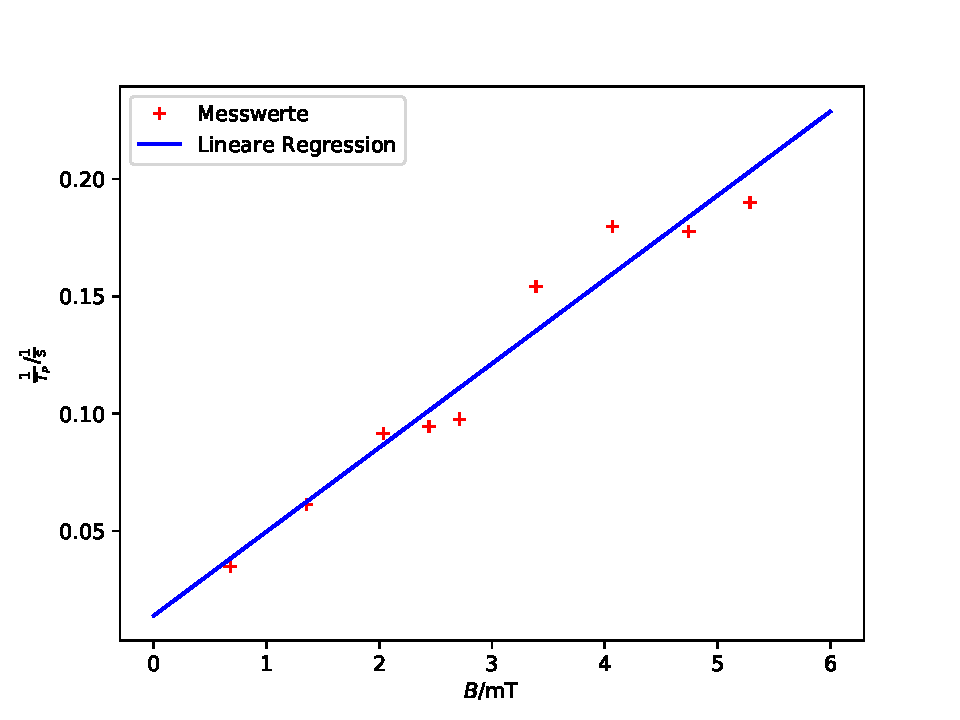
\includegraphics[scale=0.7]{Praeze.pdf}
  \caption{Messwerte und lineare Regression der Methode über Präzession}
  \label{Abb:3}
\end{figure}

Analog wie bei den anderen beiden Methoden, wird hierbei das magnetische Moment über die Steigung der linearen Regression berechnet. Aus

\begin{equation*}
  m_3 = \frac{\mu_\symup{Dipol3}}{2 \pi L_k} = \frac{\mu_\symup{Dipol3}}{2 \pi^2 J_k f}
\end{equation*}

folgt direkt

\begin{equation*}
  \mu_\symup{Dipol3} = \frac{4 \pi\squared J_k}{m_3}.
\end{equation*}

Durch Einsetzen der Steigung $m_3$ durch die lineare Regression, ergibt sich das magnetische Moment des Dipols

\begin{equation*}
  \mu_\symup{Dipol3} = \SI{28.62(248)e-2}{\ampere\meter\squared}
\end{equation*}


\section{Diskussion}

Die drei errechneten magnetischen Momente im Vergleich:

\begin{table}
  \centering
  \caption{Vergleich der magnetischen Momente}
  \label{Vergleich}
  \begin{tabular}{c c}
    \toprule
    Methode & $\mu_\symup{Dipol}$ / \si{\ampere\meter\squared} \\
    \midrule
    1 & \num{30.35(137)e-2} \\
    2 & \num{27.67(93)e-2} \\
    3 & \num{28.62(248)e-2} \\
    \bottomrule
  \end{tabular}
\end{table}

Zu erkennen ist, dass es kleine Abweichungen bei den berechneten Werten gibt. Diese sind auf die Ungenauigkeit der Messungen zurückzuführen.
Zum Beispiel bei der ersten Methode ist nicht eindeutig zu erkennen, wann sich der Stab in der Kugel nicht mehr in der vertikalen Richtung bewegt, sondern
nurnoch in der horizontalen.

Bei der zweiten Messreihe, also durch die Messung der Periodendauer, gib es auch Fehlerquellen. Eine davon ist dass 10
Periodendauern gemessen werden sollte, sobald man das Magnetfeld angestellt hat. Die Schwingung konnte man somit durch einen ungedämpften harmonischen
Oszillator annähern, aber in der Realität ist immer eine kleine Dämpfung vorhanden. Diese konnte zwar durch das Luftkissen reduziert,
aber nicht vollständig entfernt werden.

Bei der dritten und letzen Methode kommen Fehler durch das Stroboskop hinzu, da es sehr schwierig ist, die Kugel in der
Frequenz des Stroboskopes rotieren zu lassen. Eine weitere Fehlerquelle ist wiederum die Zeit, denn auch diese Bewegung ist gedämpft und somit bei
längerer Dauer ungenau. Dies wurde damit einigermaßen behoben, indem die Präzessionsbewegung direkt gestartet wurde, als die Rotationsfrequenz
erreicht wurde.

Dennoch ist zu sehen, dass die Werte verhältnismäßig nah beieinander liegen.

\newpage
\nocite{*}
\printbibliography
